\chapter{Barreiras para contribuir com software \\público}
\label{barreiras_publico}

Como explicado no Capítulo~\ref{metodologia} foi enviado o questionário, 
presente no Anexo~\ref{anexo b}, através da mensagem do Anexo~\ref{anexo a} 
enviada na lista de duscussão das 6 comunidades de software público com 
a intenção de que os desenvolvedores das comunidades respondessem. Após 2 
meses com o questionário aberto, obtivemos 19 respostas que puderam ser 
utilizadas na pesquisa sendo assim dividida entre os projetos:

\begin{table}[h]
	\centering
	\begin{tabular}{ccc}
		\toprule
		\textbf{Projeto} & \textbf{Quantidade de respostas} \\
		\midrule
		Noosfero.gov & 5 \\
		CACIC & 2 \\
		SAE & 1 \\
		I-Educar & 3 \\
		E-SIC & 3 \\
		SEI & 5 \\
		\bottomrule
	\end{tabular}

	\caption{Quantidade de respostas dos desenvolvedores por projetos.}
	\label{tab01}
\end{table}
  

Enviamos também o questionário do Anexo~\ref{anexo e} para os gestores das 
comunidades enviando a mensagem do Anexo~\ref{anexo d} para seus e-mails mas 
obtivemos apenas 3 respostas.

\begin{table}[h]
	\centering
	\begin{tabular}{ccc}
		\toprule
		\textbf{Projeto} & \textbf{Quantidade de respostas} \\
		\midrule
		Noosfero.gov & 0 \\
		CACIC & 1 \\
		SAE & 0 \\
		I-Educar & 1 \\
		E-SIC & 1 \\
		SEI & 0 \\
		\bottomrule
	\end{tabular}

	\caption{Quantidade de respostas dos coordenadores por projetos.}
	\label{tab02}
\end{table}



Na primeira fase da pesquisa, nós identificamos os conceitos com base nos dados 
dos questionários respondidos pelos desenvolvedores e pelos gestores das comunidades de
sofware público, chegamos a estes conceitos identificando de resposta em resposta 
do questionário aquilo que era identificado como barreira para desenvolver 
software público.

De acordo com as respostas dadas às perguntas na parte do perfil nós extraímos
que para 90\% dos desenvolvedores que responderam ao questionário estavam 
em seu primeiro projeto de software público e entre os gestores do projetos
100\% dos que responderam. Também percebemos que apenas
40\% eram pagos para desenvolver software público que coincidentemente ou não
40\% tinham o projeto de software público como sua principal ocupação.

Os conceitos foram extraidos conforme apareciam nas respostas dos questionários.
Algumas questões se sobressairam com relação a semelhança nas respostas, como 
por exemplo quando perguntado ``Qual era o seu conhecimento em software público 
quando você iniciou no projeto?'', 18 das 19 respostas ao questionário, os desenvolvedores
responderam que seu conhecimento era básico, nenhum ou pouco. Destas respostas 
nós conseguimos, com certeza, afirmar que a ``Falta de conhecimento em software público''
é uma barreira.

Houveram respostas bastante completas em que conseguimos extrair mais de uma barreira,
por exemplo, quando perguntado ``Como é a receptividade do projeto'' um desenvolvedor
respondeu: ``Boa, mas complicada. Muitas vezes o software não está completo, está em uma 
fase, digamos que, beta. Por esse motivo, a parte de configuração e instalação 
do software é algo mais manual, e não automatizado. Por falta de conhecimento, 
não só técnico mas do software também, a comunidade muitas fezes ficam frustradas 
apontando bugs que na verdade são apenas trabalho incompleto, que inclusive 
causaria retrabalho se feito antes do término do beta. Mas é bom, pois quanto mais 
a comunidade informa dessas dificuldades e relata bugs, mais fácil para escalar a 
importância das tarefas.''. Desta resposta conseguimos extrair algumas barreiras 
como ``Falta de informação em relação à fase do projeto'', ``Falta de lista de tarefas/
necessidades do projeto'' e ``Falta de manual de implantação do projeto''.

No contexto da entrada no projeto quando perguntado no questionário se o desenvolvedor
sabia o que fazer 9 das 19 respostas foram de que não sabiam, desta forma chegamos as
barreiras ``Não sabia por onde começar'', ``Falta de um guia de como começar'' e ``Falta de 
informação de como contribuir''. Em contrapartida obtivemos uma resposta interessante 
quando perguntado aos gestores o que ele acha a respeito da entrada de novos contribuidores
nos projetos, nos foi respondido ``Acho que devemos recebê-los e fazer de tudo 
para que tenham uma experiência positiva, encontrem documentação e acesso fácil ao 
software e principalmente, que possam deixar de alguma maneira contribuições também.''

Da maneira relatada acima chegamos a um lista inicial de 62 barreiras para desenvolver
software público. 

\begin{itemize}
\item Falta de conhecimento em software público.
\item Falta de conhecimento em software livre.
\item Não saber a diferença entre software livre e público.
\item Peculiaridades das comunidades de software público.
%
\item Desenvolvedores não escolheram estar desenvolvendo o projeto, lhes foi imposto.
\item Obrigação de manter o software no órgão em que trabalha.
\item Hierarquia do órgão.
\item Deixa de desenvolver ao sair do órgão.
%
\item Não sabia por onde começar.
\item Falta de um guia de como começar.
\item Falta de informação de como contribuir.
\item Falta de um manual de como contribuir com o projeto que indicasse o que fazer.
\item Falta de conhecimento nas práticas de desenvolvimento colaborativo.
%
\item Falta de documentação do projeto.
\item Falta de documentação para levantar ambiente.
\item Documentação confusa.
\item Falta de documentação de código.
\item Falta de manual de implantação do software e casos de sucesso em órgãos.
\item Dificuldade de encontrar a documentação do projeto.
%
\item Dificuldade de encontrar repositório oficial.
\item Informação descentralizada.
\item Falta de informações técnicas sobre o projeto.
\item Falta de informação sobre a real aplicação do projeto.
\item Falta de informação em relação à fase do projeto.
\item Falta de informações gerais sobre o projeto.
\item Apresentar os objetivos do projeto de forma clara.
%
\item Falta de lista de necessidades/tarefas do projeto.
\item Falta de canal para reportar erros e bugs no projeto.
\item Mapeamento do nível de dificuldade das tarefas do projeto.
\item Acesso às tarefas do projeto.
\item Organização das tarefas no repositório.
%
\item Falta de suporte a dificuldades.
\item Falta de mentores/líderes nos projetos para auxiliar nas dúvidas.
\item Mal uso dos fóruns de dúvidas.
\item Falta de um canal de comunicação entre os desenvolvedores.
\item Timidez para entrar em contato com a comunidade.
\item Receio em não ser bem recebido pela comunidade.
\item Falta de interação da comunidade.
\item Políticas de uso do fórum de discussão.
\item Dificuldade em lidar com pessoas de outras áreas de formação.
\item Respeito aos diferentes pontos de vista detro do projeto.
%
\item Dificuldade em encontrar normas de uso do portal SPB.
\item Dificuldade de encontrar as normas de compartilhamento de projetos no portal SPB.
\item Dificuldade de interação com os mantenedores do SPB.
\item Dificudade em entender a estrututura do SPB.
\item Dificuldade em entender as funcionalidades do portal SPB.
%
\item Falta de incentivo para retornar as contribuições feitas no projeto para a comunidade.
\item Dificuldade em enviar a melhoria para a comunidade.
\item Falta de padrões de código claros na comunidade para que as melhorias sejam aceitas.
%
\item Dificuldade com ferramenta de controle de versão.
\item Nível de conhecimento em programação.
\item Falta de conhecimentos técnicos.
%
\item Má qualidade do código.
\item Código confuso.
\item Código com muitos erros.
\item Imaturidade do código.
%
\item Dedicação ao projeto.
\item Motivação social.
\item Motivação apenas financeira para contribuir com o software.
\item Proatividade.
\item Comprometimento com o projeto.
\item Colocar os objetivos do projeto à frente dos seus objetivos pessoais com o projeto.
%

\end{itemize}

Após a identificação dos conceitos, partimos para a segunda fase apresentada pela
\textit{Ground Theory}, que como explicado no Capítulo \ref{barreirasSL}, demanda que  
façamos a categorização dos conceitos agrupando os conceitos relacionados. Para esta 
atividade, primeiramente, separamos as barreiras em grupos por semelhança e assunto,
dessa forma conseguimos avaliar se haviam barreiras se repetindo ou muito parecidas
semanticamente e tranformá-las em uma única barreira. Após esta análise obtivemos 6 
grupos que posteriormente definimos como categorias quando já havíamos determinado
nomes para as mesmas. 

Com a categorização destes grupos, percebemos ainda que algumas das categorias
poderiam ter uma subcategorização para que o modelo ficasse mais claro e remover
algumas redundâncias, dessa forma chegamos a 50 barreiras mapeadas com as categorias
descritas a seguir.


\begin{figure}[h]
	\centering
	\label{fig:SPbarreiras}
		\includegraphics[keepaspectratio=true,scale=0.3]{figuras/Barreiras_Software_Publico_.eps}
	\caption{Barreiras para contribuir com Software público.}
\end{figure}


\begin{enumerate}
\item \textbf{Conhecimento em software livre e público}, nós descobrimos que quando
o desenvolvedor se dispõe a contribuir com software público muitas das vezes ele
não sabe o que isso significa, os desenvolvedores não
tem conhecimento do que implica no desenvolvimento as características inerentes
a estes tipos de projetos. Existe também uma dificuldade de entender a estrutura
e as funcionalidades do portal SPB, além da dificuldade em contactar a equipe de 
mantenedores do portal. Os novos desenvolvedores precisam ter um treinamento para entender
o que significa dizer que o um software é público ou livre além de conseguir contactar os
adminitradores do portal para tirar eventuais dúvidas.
Para desenvolvedores que se tornam Analistas de Tecnologia da Informação esta 
capacitação deve ser dada no curso de formação, desta forma, ao iniciar o cumprimento
de suas funções estes conceitos e a operação do portal SPB não serão mais um problema.

\item \textbf{Hierarquia}, nós observamos que a hierarquia dentro dos órgãos públicos 
dificulta o desenvolvimento de softwares públicos, pois eles são obrigados a desenvolver
ou manter o software dentro dos seus órgãos mas quando o servidor deixa o órgão ou aquele 
deixa de ser prioridade o servidor é desencorajado a continuar contribuindo com o projeto.
Deveriam haver políticas públicas dentro dos órgãos para incentivar o desenvolvimento de 
projetos software público, sabendo que os sofware públicos são consultados antes de se
desenvolver um projeto de software pelo governo. 

\item \textbf{Orientação a novos desenvolvedores}, nós conseguimos observar que os 
novos desenvolvedores precisam de orientações para começar a contribuir, desde como
começar até que tarefas ele pode fazer para que não fique desmotivado devido ao grau
de dificuldade de uma tarefa.

\item \textbf{Documentação}, a falta de documentação do projeto demonstrou ser um
problema em alguns projetos, pela falta de documentação ou quando presente, por estar descentralizada 
ou até mesmo confusa e o novo desenvolvedor não consegue acha-la ou entendê-la. Os novos 
desenvolvedores precisam de uma documentação clara para os ajudar a entender e contribuir
com o projeto. A criação de \textit{workshops} dos projetos onde os desenvolvedores
possam se encontrar e trocar experiências ajudaria no entendimento do projeto pelos
novatos além de treinamentos específicos para os projetos. Como exemplo o projeto
SEI\footnote{https://softwarepublico.gov.br/social/sei} que oferece, através da
ENAP, cursos de capacitação no projeto presenciais e à distancia.

\item \textbf{Dificuldades técnicas}, os novos desenvolvedores tem dificuldade em dar os
primeiros passos em relação as tarefas técnicas do projeto como levantar o ambiente e até
mesmo encontrar o repositório oficial do projeto, o código também é dificil de entender
na maioria dos projetos de sofware público por não haver um padrão de codificação, além de 
os novos desenvolvedores não conhecerem a linguagem e as ferramentas que irão precisar trabalhar.
Deveria ficar claro para os novos desenvolvedores quais as tecnologias que eles 
devem conhecer para contribuir com o projeto além de um tutorial claro de como levantar 
o ambiente da aplicação para que fique possível o estudo do código.

\item \textbf{Características dos novos contribuidores}, nós observamos que o comportamento 
dos novos desenvolvedores é um fator crucial para o sucesso do mesmo no projeto, é necessario
que ele seja proativo, dedicado e tenha comprometimento com o projeto para obter sucesso
em sua contribuição. A maneira com que o novo desevolvedor utiliza as listas de e-mail
também influencia a atenção que os mantenedores do projeto irão desprender ao novo
desenvolvedor. O conhecimento do novo desenvolvedor em ferramentas de controle de versão
é necessário para que o novo desenvolvedor contribua com qualquer projeto que adote este
modelo de desenvolvimento, conhecimento em liguagens de programação pode limitar o quanto ele 
vai conseguir contribuir com a comunidade.

\end{enumerate}

\section{Análise comparativa com as barreiras conhecidas de Software Livre}

Como já mencionamos, projetos de software livre e público tem características 
diferentes embora tenha muitas semelhanças, desta forma é esperado que entre as
barreiras encontradas para os dois tipos de projetos nós tenhamos também pontos 
em que as barreiras sejam equivalentes e pontos que sejam barreiras apenas para
um tipo de projeto.

A primiera categoria relatada na pesquisa do professor Igor é a chamada \textbf{Tarefas
de recepção} e engloba as barreiras: Não obtenção de resposta, resposta atrasada e
resposta mal educada. Na nossa pesquisa não encontramos aplicação para esta categoria,
não houve pelos desenvolvedores ou gestores de projetos, nenhum relato a respeito das 
barreiras citadas.

A categoria \textbf{Conhecimento em software livre e público} se aplica apenas a
barreiras para projetos de software público pela razão de que um desenvolvedor 
que deseje contribuir apenas com projetos de software livre não tem a necessidade 
de conhecer a respeito de software público mas o contrário não se aplica, aquele 
desenvolvedor que pleita contribuir com projetos de software público se sente
mais confortável em também saber as característcas de software livre. Atribuímos
esta barreira também uma consequência da próxima categoria que iremos mencionar, 
\textbf{Hierarquia}, como os desenvolvedores não escolhem o projeto com o qual irão
contribuir eles acabam não tendo o tempo necessário para aprender previamente quais
são características dde um projeto de software público ou livre.

\begin{figure}[h]
	\centering
	\label{fig:conhecimentos}
		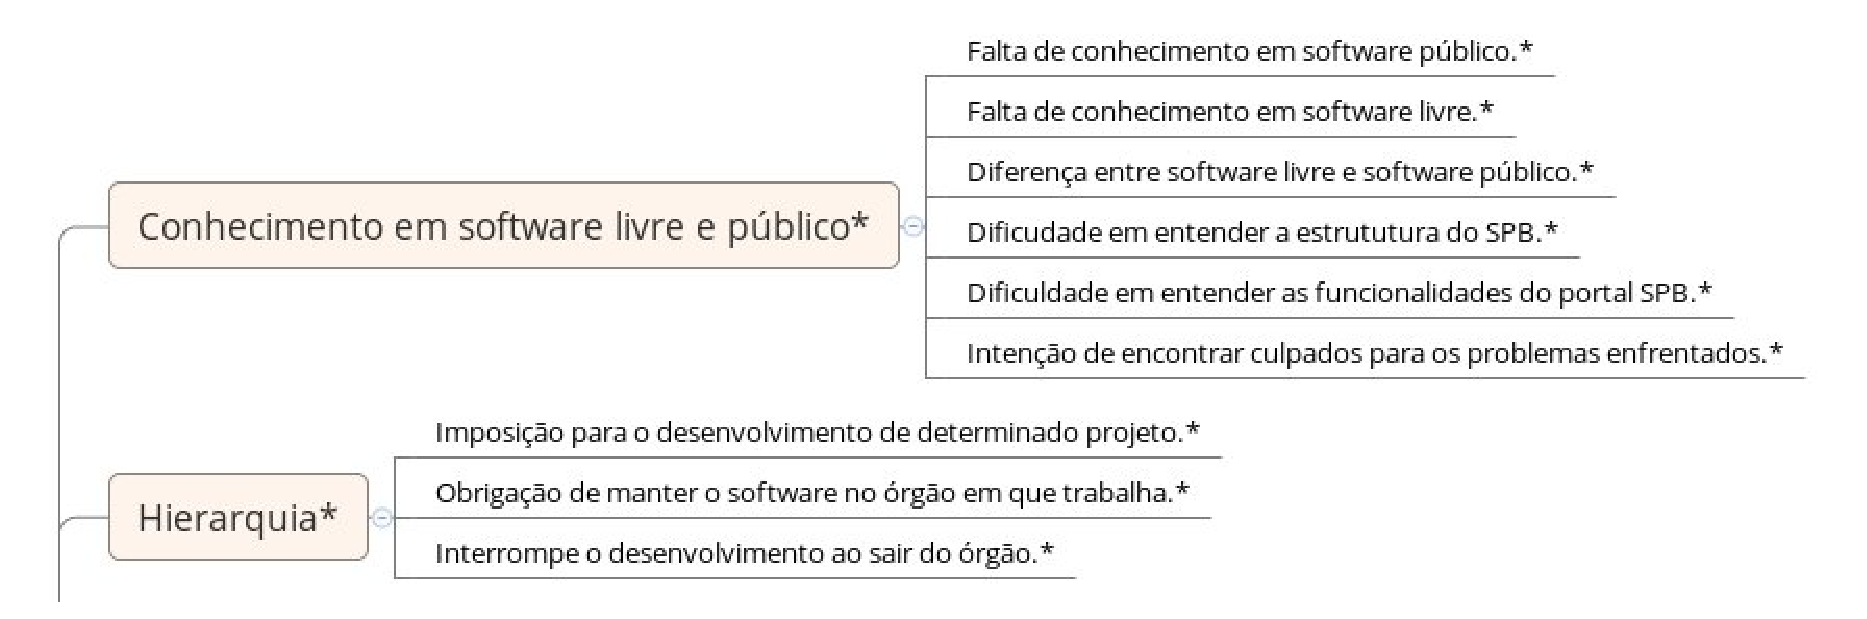
\includegraphics[keepaspectratio=true,scale=0.5]{figuras/conhecimentos.eps}
	\caption{Categorias Conhecimentos em software livre e público e Hierarquia.}
\end{figure}

A \textbf{Hierarquia} é uma categoria e característica apenas de projetos de
software livre. Em projetos de software livre o desenvolvedor tem a oprtunidade
de escolher se quer fazer parte daquele projeto ou não ao contrário do software
público que muitas das vezes o desenvolvedor passa a fazer parte do projeto por
uma delegação de superiores no órgão do governo em que trabalha.

As \textbf{Diferenças culturais} que se apresenta como uma categoria das barreiras
para software livre já não se aplica a software público. Não houveram relatos de que alguém 
considerou uma mensagem rude ou necessitou de contato com os desenvolvedores do projeto.
Isso se dá primeiramente porque estamos tratando de software público brasileiro que 
é uma coisa que está voltalda apenas para desenvolvedores em nosso país, sendo assim
não há a preocupação de que alguém que não tenha a nossa cultura vá se ofender com a 
mensagem. Outra característica é a de que os desenvolvedores de software público quase
sempre trabalham na mesma equipe e ambiente físico que outros desenvolvedores do mesmo 
projeto, facilitando assim o contato pessoal.

\begin{figure}[h]
	\centering
	\label{fig:caracteristicas}
		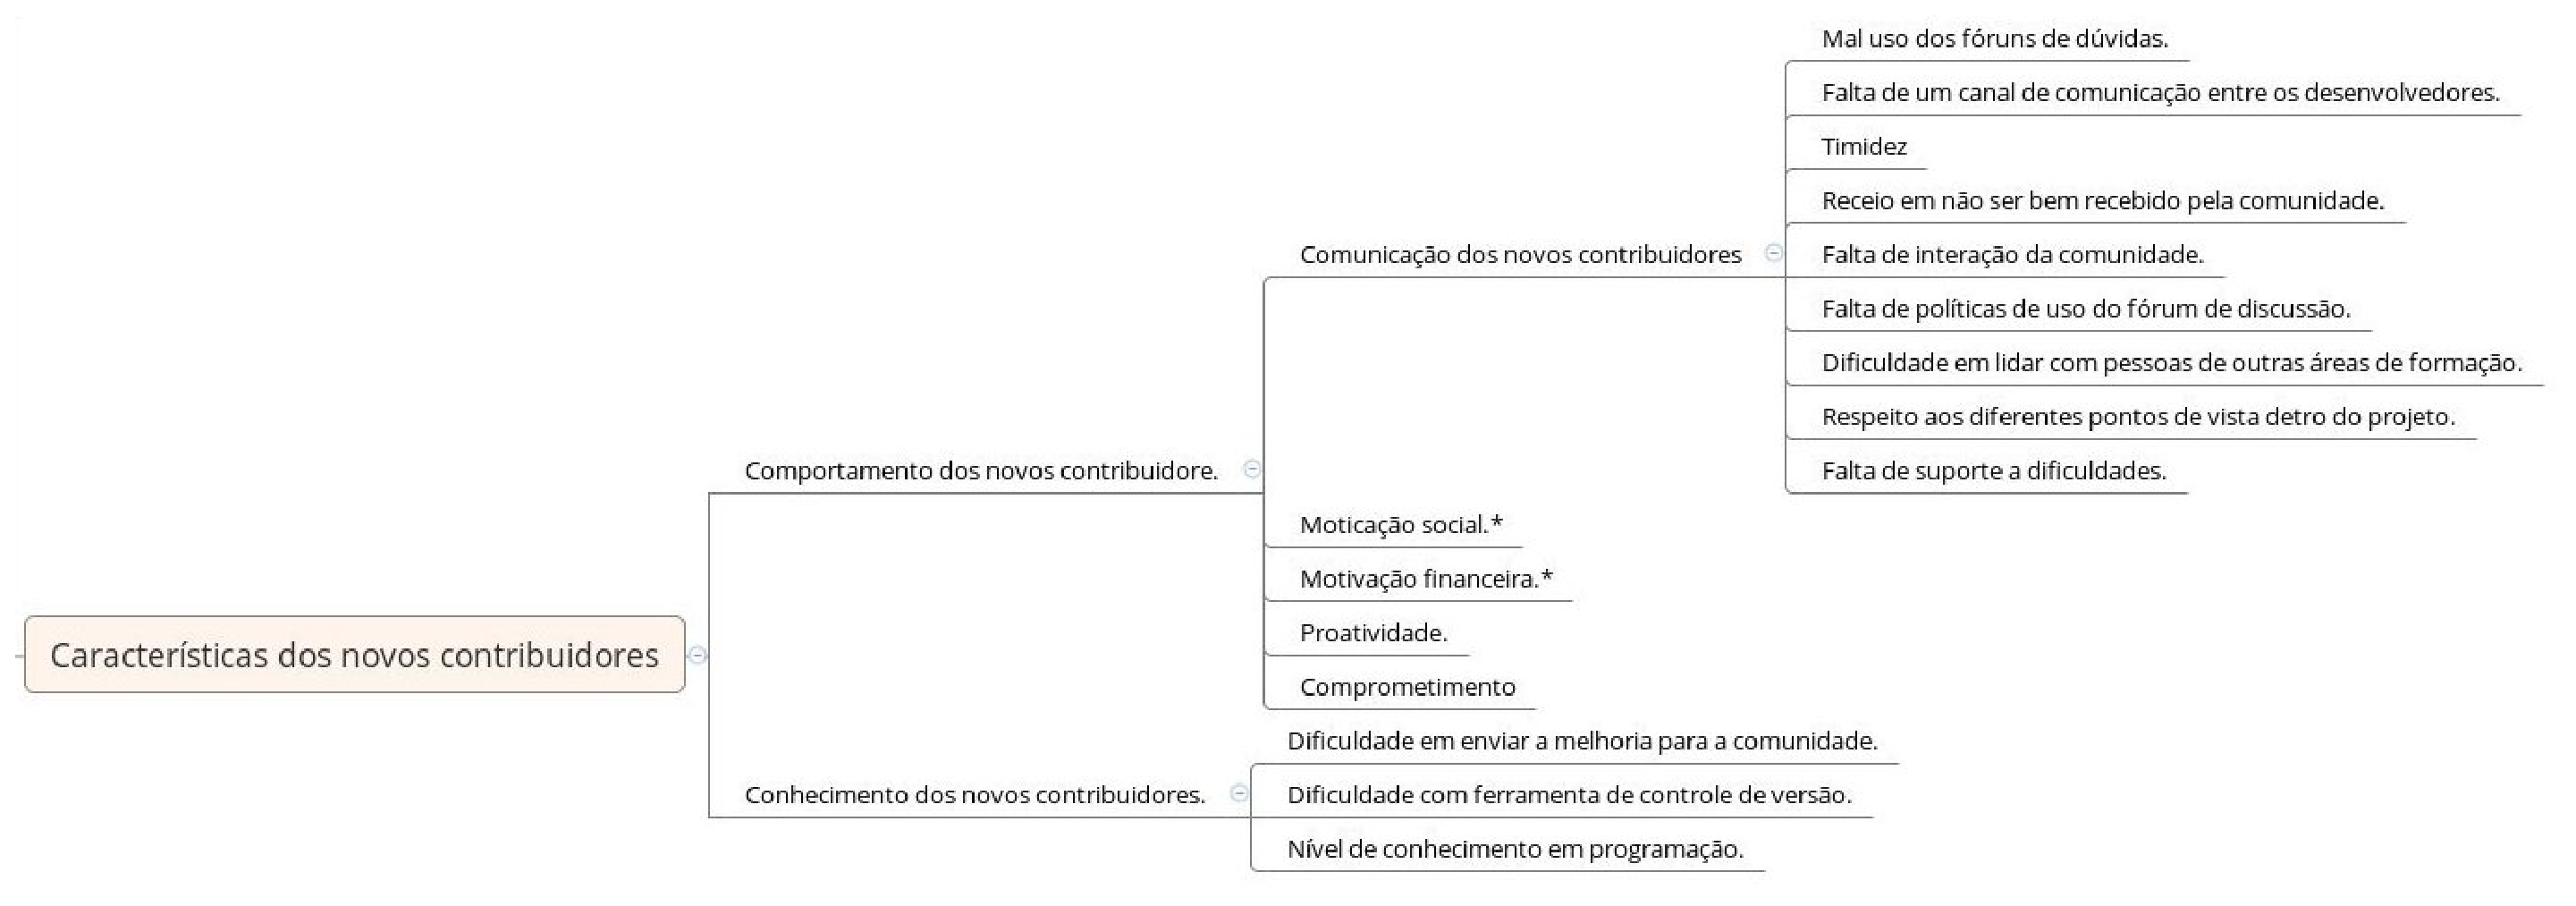
\includegraphics[keepaspectratio=true,scale=0.35]{figuras/caracteristicas.eps}
	\caption{Categoria Caracterísicas dos novos contribuidores.}
\end{figure}

\begin{figure}[h]
	\centering
	\label{fig:documentacao}
		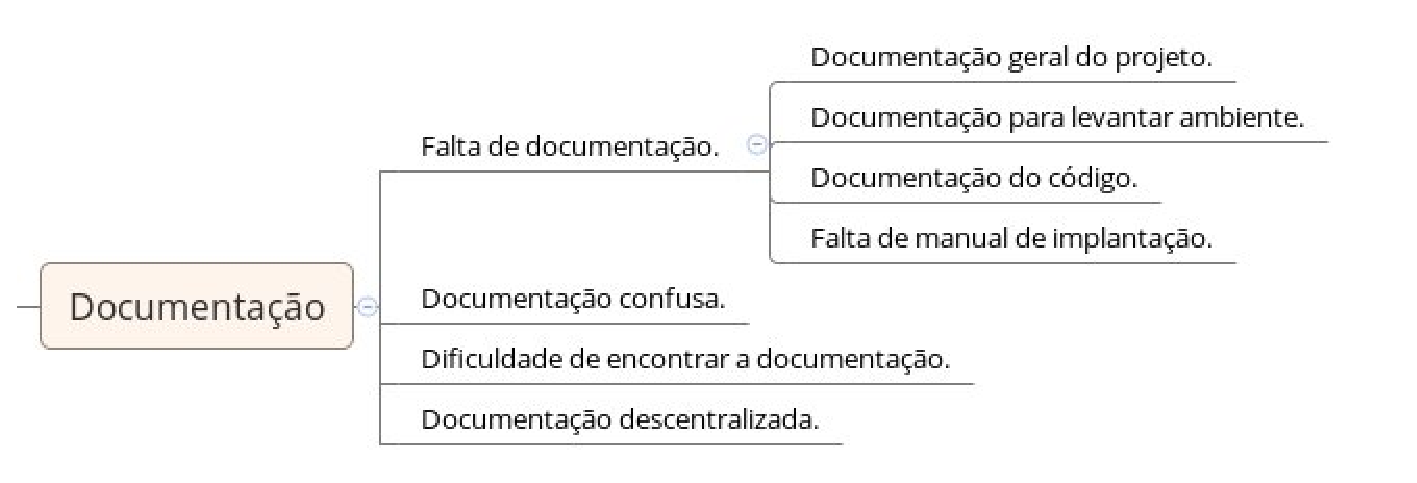
\includegraphics[keepaspectratio=true,scale=0.5]{figuras/documentacao.eps}
	\caption{Categoria Documentação.}
\end{figure}

\begin{figure}[h]
	\centering
	\label{fig:dificuldades}
		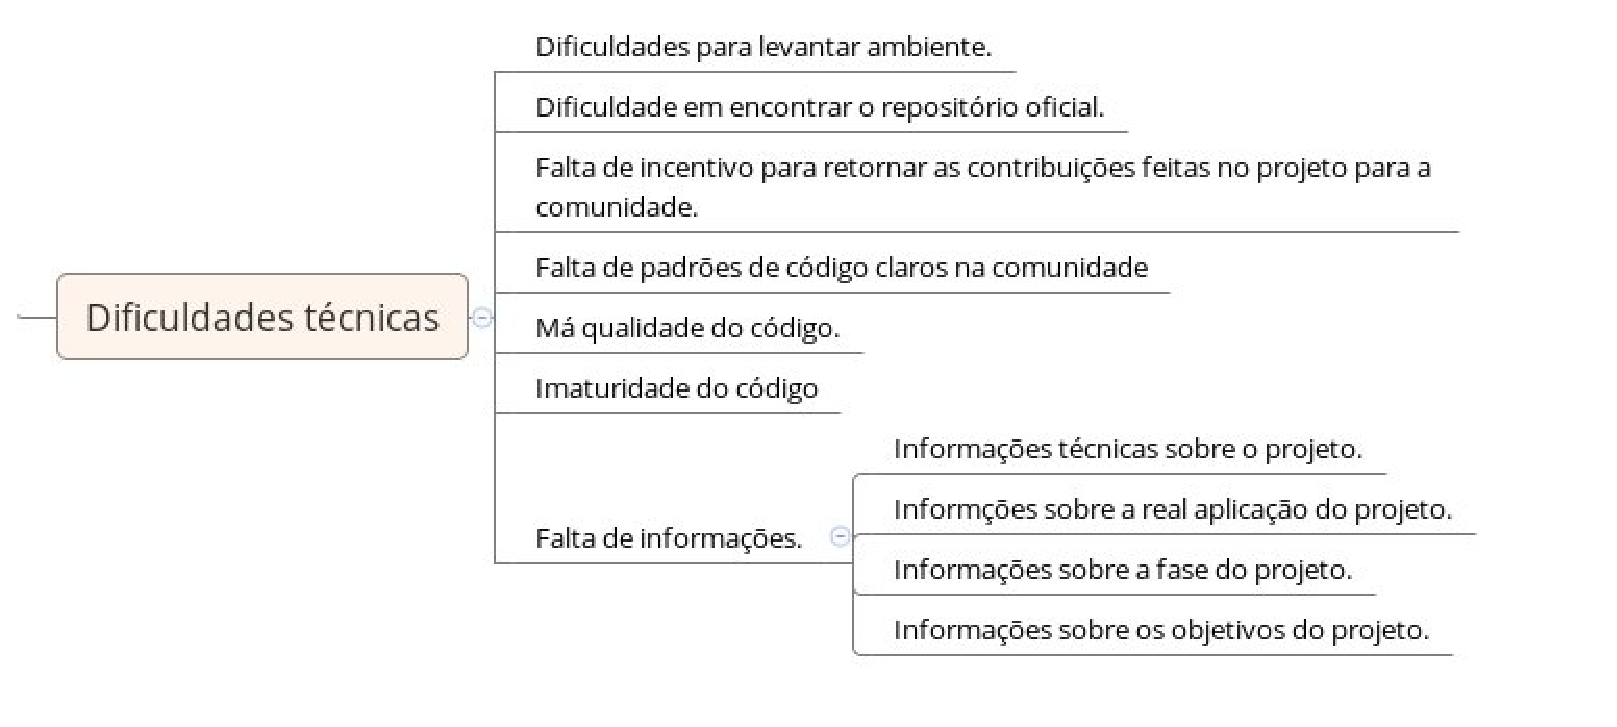
\includegraphics[keepaspectratio=true,scale=0.5]{figuras/dificuldades.eps}
	\caption{Categoria Dificuldades técnicas.}
\end{figure}

As mesmas \textbf{Características dos novos contribuidores} encontradas nas barreiras
de software livre foram encontradas para software público com excessão apenas de duas
motivações, social e financeira, que se destacaram nas barreiras para software público.
A motivação social se dá por alguns desenvolvedores acreditarem que ao contribuir com 
software público estão fazendo sua parte para melhorar o país em suas esferas, já
a motivação financeira é exclusivamente pelo motivo de que alguns desenvolvedores
desenvolvem software livre pelo retorno financeiro que tem em seus projetos.


Os mesmos problemas com \textbf{Documentação} enfrentados pelos desenvolvedores de 
projetos de software público são também vistos por aqueles que desenvolvem software 
livre. Documentação incompleta, descentralizada e faltando são reclamações comuns aos
diferentes tipos de projetos.

As \textbf{Dificuldades técnicas} é outro ponto de interseção entre os dois tipos
de projeto. Levantar ambiente, má qualidade do código e entendimento do código
não é tarefa fácil para quem esta entrando nos projetos. O que se apresenta ser
os mesmos problemas para software livre e público para software público é ainda
mais grave, quando fazemos uma ligação com as \textbf{Características dos novos contribuidores}
observamos que aparentemente os desenvolvedores que começam a contribuir com software
público tem um conheciemnto técnico inferior àqueles que iniciam contribuição em 
projetos de software livre, o que dificulta ainda mais a entrada dos desenvolvedores.

\begin{figure}[h]
	\centering
	\label{fig:orientacoes}
		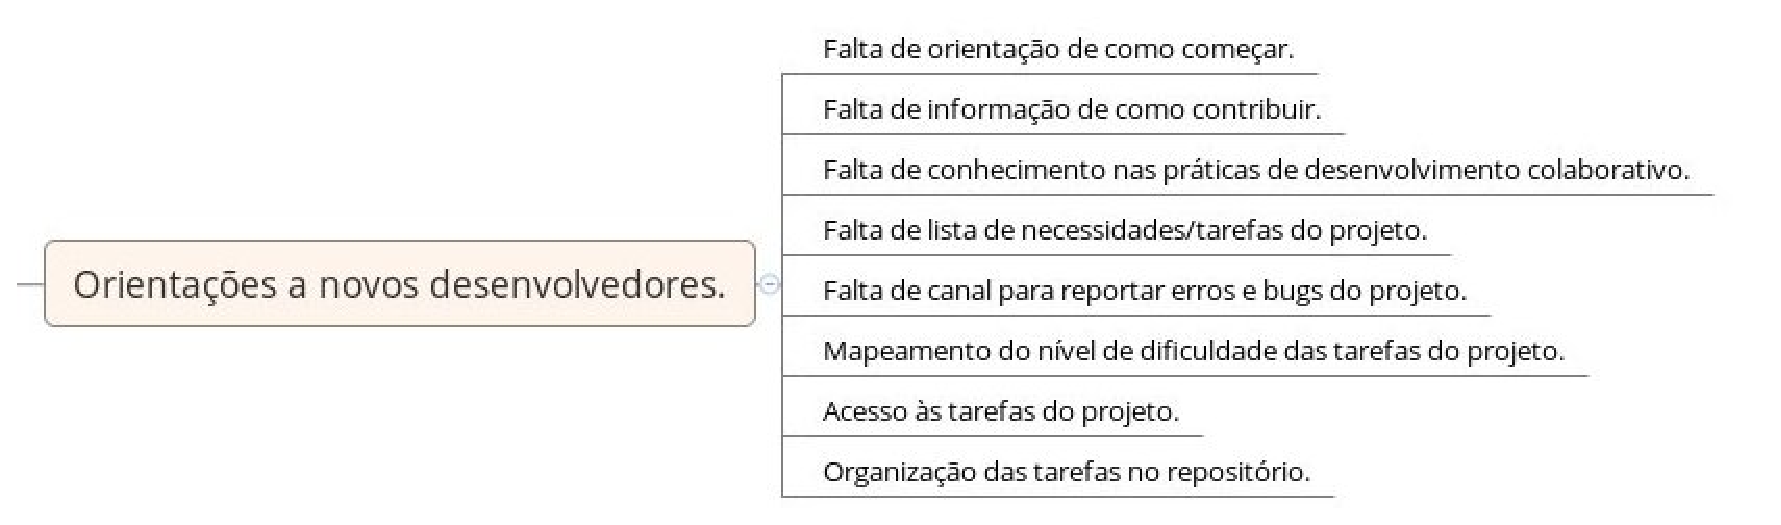
\includegraphics[keepaspectratio=true,scale=0.5]{figuras/orientacoes.eps}
	\caption{Categoria Orientações aos novos desenvolvedores.}
\end{figure}

Levando em consideração os pontos citados acima, nós conseguimos abstrair o que
ficou claro na pesquisa, os novos contribuidores dos dois tipos de projetos precisam
basicamente das mesmas \textbf{Orientações a novos contribuidores}, como começar é 
uma dificuldade enfrentada pelos novos desenvolvedores nos projetos seja de 
software livre ou software público. Dessa forma podemos afirmar que o
FlossCoach consegue auxiliar tanto desenvolvedores que iniciam em projetos de software
livre quanto público e com o desenvolvimento do novo portal FlossCoach um maior
número de novos desenvolvedores serão ajudados a iniciar suas contribuições.


